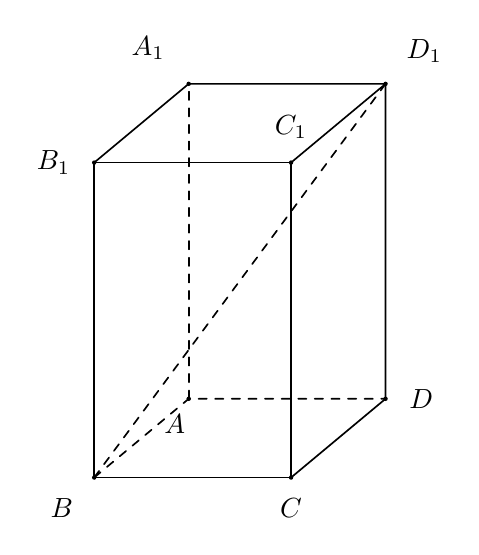
\begin{tikzpicture}[line width=0.6pt, line join=round, line cap=round]
\coordinate (B) at (0,0);
\coordinate (C) at (2.5,0);
\coordinate (A) at (1.2,1.0);
\coordinate (D) at (3.7,1.0);
\coordinate (B1) at (0,4);
\coordinate (C1) at (2.5,4);
\coordinate (A1) at (1.2,5.0);
\coordinate (D1) at (3.7,5.0);
% front face solid
\draw (B) -- (C) -- (C1) -- (B1) -- cycle;
% top face solid
\draw (B1) -- (A1) -- (D1) -- (C1);
% right face solid
\draw (C) -- (D) -- (D1);
% right vertical D-D1 already above; front-right vertical C-C1 part of front face
% hidden bottom / back edges dashed
\draw[dashed] (B) -- (A) -- (D);
\draw[dashed] (A) -- (A1);
\draw[dashed] (B) -- (D1);
\foreach \p in {A,B,C,D,A1,B1,C1,D1} {\fill (\p) circle (0.8pt);}
\node[below left=4pt] at (B) {$B$};
\node[below=4pt] at (C) {$C$};
\node[left=5pt,below=2pt] at (A) {$A$};
\node[right=5pt] at (D) {$D$};
\node[left=5pt] at (B1) {$B_{1}$};
\node[above left=5pt] at (A1) {$A_{1}$};
\node[above=5pt] at (C1) {$C_{1}$};
\node[above right=4pt] at (D1) {$D_{1}$};
\end{tikzpicture}
